% Options for packages loaded elsewhere
\PassOptionsToPackage{unicode}{hyperref}
\PassOptionsToPackage{hyphens}{url}
\PassOptionsToPackage{dvipsnames,svgnames,x11names}{xcolor}
\PassOptionsToPackage{space}{xeCJK}
\documentclass[
  10pt,
]{article}
\usepackage{xcolor}
\usepackage[margin=0.72in]{geometry}
\usepackage{amsmath,amssymb}
\setcounter{secnumdepth}{-\maxdimen} % remove section numbering
\usepackage{iftex}
\ifPDFTeX
  \usepackage[T1]{fontenc}
  \usepackage[utf8]{inputenc}
  \usepackage{textcomp} % provide euro and other symbols
\else % if luatex or xetex
  \usepackage{unicode-math} % this also loads fontspec
  \defaultfontfeatures{Scale=MatchLowercase}
  \defaultfontfeatures[\rmfamily]{Ligatures=TeX,Scale=1}
\fi
\usepackage{lmodern}
\ifPDFTeX\else
  % xetex/luatex font selection
  \setmainfont[]{Arial}
  \setmonofont[]{Consolas}
  \ifXeTeX
    \usepackage{xeCJK}
    \setCJKmainfont[]{Microsoft YaHei}
  \fi
  \ifLuaTeX
    \usepackage[]{luatexja-fontspec}
    \setmainjfont[]{Microsoft YaHei}
  \fi
\fi
% Use upquote if available, for straight quotes in verbatim environments
\IfFileExists{upquote.sty}{\usepackage{upquote}}{}
\IfFileExists{microtype.sty}{% use microtype if available
  \usepackage[]{microtype}
  \UseMicrotypeSet[protrusion]{basicmath} % disable protrusion for tt fonts
}{}
\makeatletter
\@ifundefined{KOMAClassName}{% if non-KOMA class
  \IfFileExists{parskip.sty}{%
    \usepackage{parskip}
  }{% else
    \setlength{\parindent}{0pt}
    \setlength{\parskip}{6pt plus 2pt minus 1pt}}
}{% if KOMA class
  \KOMAoptions{parskip=half}}
\makeatother
\usepackage{longtable,booktabs,array}
\usepackage{calc} % for calculating minipage widths
% Correct order of tables after \paragraph or \subparagraph
\usepackage{etoolbox}
\makeatletter
\patchcmd\longtable{\par}{\if@noskipsec\mbox{}\fi\par}{}{}
\makeatother
% Allow footnotes in longtable head/foot
\IfFileExists{footnotehyper.sty}{\usepackage{footnotehyper}}{\usepackage{footnote}}
\makesavenoteenv{longtable}
\usepackage{graphicx}
\makeatletter
\newsavebox\pandoc@box
\newcommand*\pandocbounded[1]{% scales image to fit in text height/width
  \sbox\pandoc@box{#1}%
  \Gscale@div\@tempa{\textheight}{\dimexpr\ht\pandoc@box+\dp\pandoc@box\relax}%
  \Gscale@div\@tempb{\linewidth}{\wd\pandoc@box}%
  \ifdim\@tempb\p@<\@tempa\p@\let\@tempa\@tempb\fi% select the smaller of both
  \ifdim\@tempa\p@<\p@\scalebox{\@tempa}{\usebox\pandoc@box}%
  \else\usebox{\pandoc@box}%
  \fi%
}
% Set default figure placement to htbp
\def\fps@figure{htbp}
\makeatother
\setlength{\emergencystretch}{3em} % prevent overfull lines
\providecommand{\tightlist}{%
  \setlength{\itemsep}{0pt}\setlength{\parskip}{0pt}}
\usepackage{bookmark}
\IfFileExists{xurl.sty}{\usepackage{xurl}}{} % add URL line breaks if available
\urlstyle{same}
\hypersetup{
  colorlinks=true,
  linkcolor={blue},
  filecolor={Maroon},
  citecolor={Blue},
  urlcolor={blue},
  pdfcreator={LaTeX via pandoc}}

\author{}
\date{}

\usepackage{float}
\usepackage{needspace}
\Urlmuskip=0mu plus 2mu\relax
\begin{document}

\section{Data expansion, fundus degradation, and evaluation
design}\label{data-expansion-fundus-degradation-and-evaluation-design}

November 13, 2026 · Eye Sentinel

\href{data-and-degradation-review.zh.md}{中文} ·
\href{data-and-degradation-review.en.pdf}{English PDF} ·
\href{../progress-overview.en.md}{Daily progress overview}

This report records the data review and experimental design completed
before the new training round on November 13. The
\href{../training-results/training-results.en.md}{training report}
documents the four subsequent arms, and the
\href{../experimental-analysis/experimental-analysis.en.md}{experimental
analysis} explains their paired results. Read the three reports in the
order of data preparation, training, and interpretation.

\subsection{Main results}\label{main-results}

The audit covered 13,176 candidate fundus photographs and admitted
\textbf{9,070 disease-labeled images, including 3,446 positives}. A
separate auxiliary pool retains 204 suspect images. Every candidate
image has a decision, and all 315,074 similarity candidate pairs were
adjudicated. Admission uses original source labels, permissions, file
integrity, and known patient and image relationships.

The expansion pool contains 146 real poor-quality positive photographs:
99 FIVES images with at least one poor-quality dimension and 47 MSHF
images with poor overall quality. These cases support evaluation of
disease recognition under real quality variation. Synthetic defocus and
exposure changes support training augmentation and paired stress
comparisons; case counts follow the original photographs.

The review proposed 0\%, 30\%, and 50\% degradation arms and recording
actual training draws from original and added sources. The later
training round used a new joint allocation of 15,480 training images,
2,046 model-validation images, and 2,053 rule-development images.
Descriptions of earlier training below refer to formal\_v3 at the review
stage. Expansion-pool counts, original-release counts, and later
training counts are kept explicit.

\subsection{1. Models and data at the review
stage}\label{models-and-data-at-the-review-stage}

The formal\_v3 EfficientNet-B0 disease model A, ResNet50 candidate B,
original quality model, and EyeQ quality model each completed 20 epochs.
A selected epoch 16 and B selected epoch 18, achieving AUROCs of 0.9766
and 0.9831 on AIROGS model validation.

AUROC is the area under the receiver operating characteristic curve. It
describes ranking: for a randomly drawn positive and negative from the
same evaluation set, it is the probability that the model assigns the
positive a higher score, counting ties as one half. A value of 0.5
corresponds to random ranking and 1.0 to perfect separation. Misses and
false positives at a chosen threshold are reported as separate counts.

The original quality model selected epoch 16. EyeQ selected epoch 17 by
combined validation loss and achieved macro-F1 0.811 on 117 human-graded
validation images in three quality categories; the final epoch 20
achieved 0.865. Macro-F1 gives equal weight to each quality category.
Selected and final-epoch results are recorded separately.

\Needspace{10\baselineskip}
\begin{longtable}[]{@{}
  >{\raggedright\arraybackslash}p{(\linewidth - 8\tabcolsep) * \real{0.1667}}
  >{\raggedleft\arraybackslash}p{(\linewidth - 8\tabcolsep) * \real{0.2222}}
  >{\raggedleft\arraybackslash}p{(\linewidth - 8\tabcolsep) * \real{0.2222}}
  >{\raggedleft\arraybackslash}p{(\linewidth - 8\tabcolsep) * \real{0.2222}}
  >{\raggedright\arraybackslash}p{(\linewidth - 8\tabcolsep) * \real{0.1667}}@{}}
\toprule\noalign{}
\begin{minipage}[b]{\linewidth}\raggedright
Set at review stage
\end{minipage} & \begin{minipage}[b]{\linewidth}\raggedleft
Images
\end{minipage} & \begin{minipage}[b]{\linewidth}\raggedleft
Positive images
\end{minipage} & \begin{minipage}[b]{\linewidth}\raggedleft
Positive linked groups
\end{minipage} & \begin{minipage}[b]{\linewidth}\raggedright
Role
\end{minipage} \\
\midrule\noalign{}
\endhead
\bottomrule\noalign{}
\endlastfoot
formal\_v3 disease training & 10,354 & 4,422 & 4,341 & Learn disease
models \\
formal\_v3 model validation & 1,190 & 489 & 482 & Select weights \\
November 13 repaired rule development & 1,220 & 503 & 494 & Calibration
and review-rule development \\
Frozen internal test & 1,233 & 489 & 481 & Evaluate after locking models
and rules \\
ACRIMA external test & 705 & 396 & 396 & External-source evaluation \\
HYGD external test & 737 & 540 & 183 & Patient/image grouped
evaluation \\
\end{longtable}

Linked groups connect known patients, paired eyes, repeated photographs,
and image versions. Sources without published patient identifiers use
image-association groups. Labels remain source-specific: AIROGS RG/NRG
describes referral for glaucoma, while other sources use their own
glaucoma diagnosis or glaucomatous optic neuropathy (GON) definitions.

\begin{figure}[H]
\centering
\pandocbounded{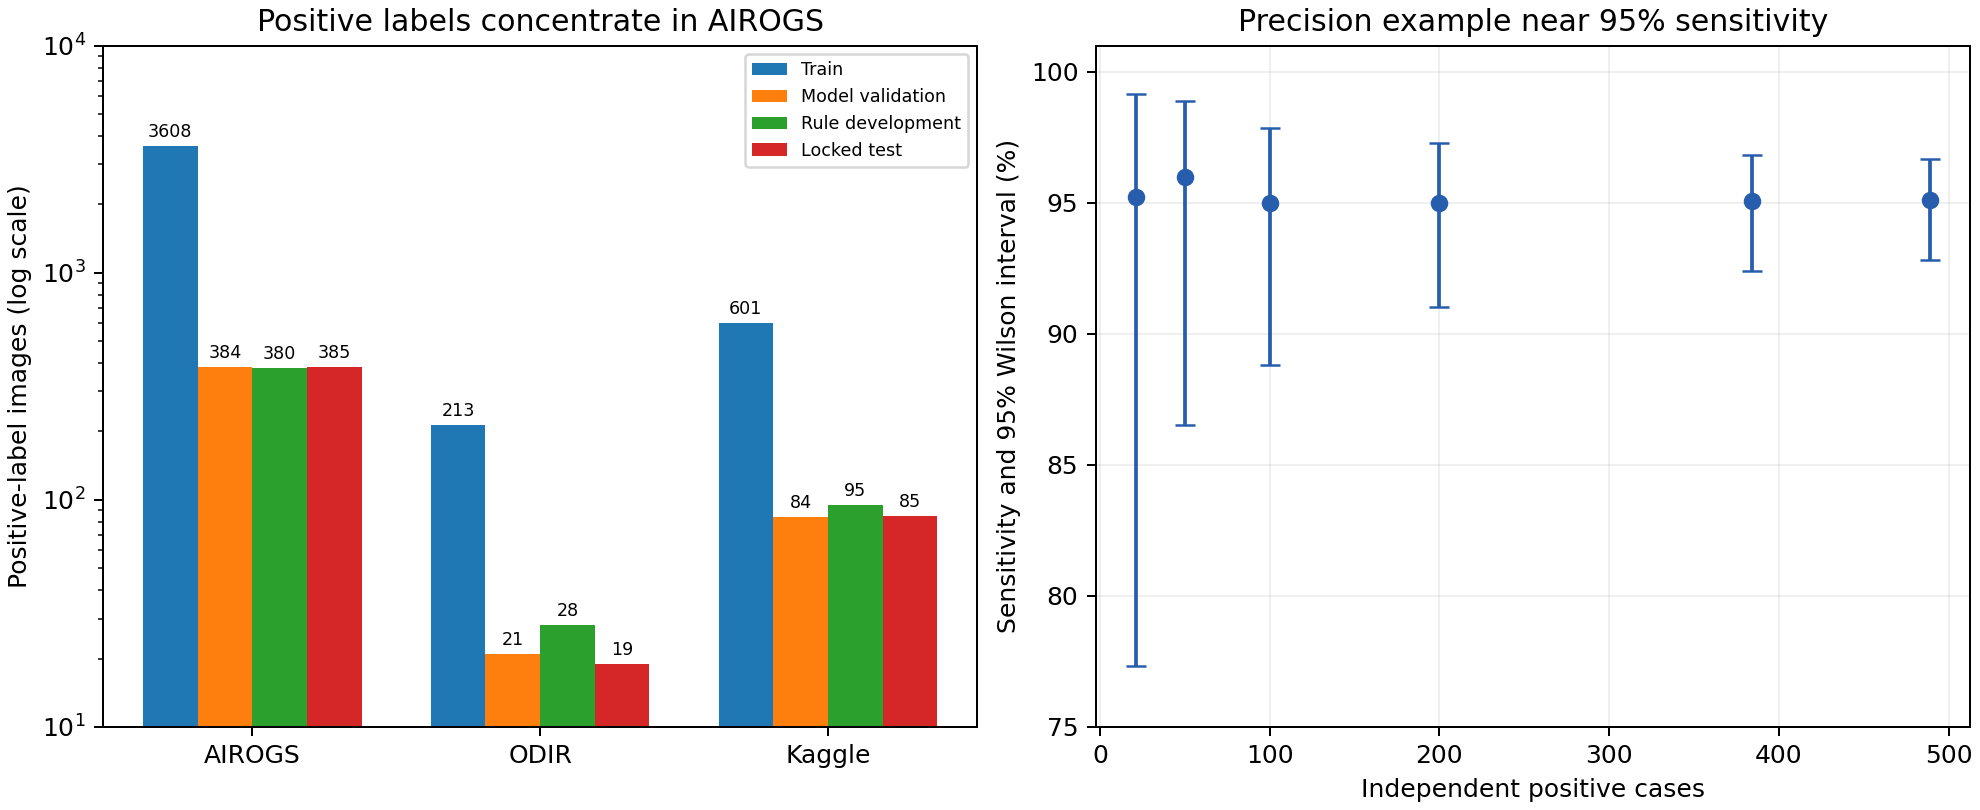
\includegraphics[keepaspectratio,alt={Original-release positive counts and sensitivity-precision examples}]{positive_counts_and_precision.png}}
\caption{Original-release positive counts and sensitivity-precision
examples}
\end{figure}

Figure 1 shows positive-image counts in four original-release roles on
the left, with a logarithmic vertical axis. Training contains 3,608
AIROGS, 601 Kaggle, and 213 ODIR positives. ODIR model validation, rule
development, and testing contain 21, 28, and 19 positives. The right
panel illustrates Wilson 95\% intervals near 95\% sensitivity to explain
how independent positive counts affect precision. Actual evaluations
account for paired eyes and repeated photographs through linked-group
resampling.

On the same 277 ODIR model-validation images, A and B achieve AUROCs of
0.9042 and 0.8950. At display threshold 0.5, A detects 13/21 positives,
with an image-level Wilson interval of approximately 40.9\%--79.2\%. The
difference from AIROGS supports source-specific evaluation; the small
positive subset also limits precision. Deployment thresholds are
determined through later model validation and rule development.

The original sampler gives equal weight to each source and each class
within a source, drawing 10,354 images with replacement per epoch. Each
source/class receives approximately 1,726 draws. An ODIR positive is
drawn 8.10 times on average, a Kaggle negative 4.87 times, and an AIROGS
positive 0.478 times. Training records therefore need update budgets,
actual draws, and distinct-image coverage.

A's mean training-batch loss falls from 0.307 to 0.027 while validation
cross-entropy rises from 0.296 to 0.435. B's training loss falls from
0.253 to 0.025 while validation cross-entropy rises from 0.367 to 0.518.
Cross-entropy measures agreement between probabilities and labels and is
particularly sensitive to confident errors. These curves motivate
comparisons of sampling, checkpoint selection, probability calibration,
and augmentation. Grouped learning curves address training size
separately.

\subsection{2. Public datasets and admission
decisions}\label{public-datasets-and-admission-decisions}

The search covered dedicated glaucoma datasets, multi-disease fundus
datasets with image-level glaucoma labels, real-quality data, catalogs,
and standardized collections, including related work from 2024--2026.
Evidence includes author papers, official releases, terms, and
obtainable images. Third-party collections are assigned to their parent
sources and deduplicated. All 45 reviewed entries appear below. DR
denotes diabetic retinopathy; OCT denotes optical coherence tomography,
a separate modality from the color fundus photographs used here.

\Needspace{10\baselineskip}
\begin{longtable}[]{@{}
  >{\raggedright\arraybackslash}p{(\linewidth - 2\tabcolsep) * \real{0.5000}}
  >{\raggedright\arraybackslash}p{(\linewidth - 2\tabcolsep) * \real{0.5000}}@{}}
\toprule\noalign{}
\begin{minipage}[b]{\linewidth}\raggedright
Source
\end{minipage} & \begin{minipage}[b]{\linewidth}\raggedright
Decision and evidence
\end{minipage} \\
\midrule\noalign{}
\endhead
\bottomrule\noalign{}
\endlastfoot
\href{https://github.com/smilell/AG-CNN}{LAG} & Official part 1
acquired: 4,854 images, 1,711 positives; clinical diagnosis established
in the original paper. Academic use; no reupload. \\
\href{https://springernature.figshare.com/articles/dataset/GRAPE_dataset_CFPs/23575926}{GRAPE}
& Originals and clinical table acquired: 144 people, 263 eyes, 631
photographs, all glaucoma. CC0. \\
\href{https://figshare.com/articles/dataset/27938034}{Fundus-AVSeg} &
Official 100-image package acquired, including 20 glaucoma images; masks
counted separately. CC BY 4.0. \\
\href{https://figshare.com/articles/dataset/LES-AV_dataset/11857698}{LES-AV}
& Official 22 images and clinical table acquired, including 11 glaucoma
images. GPL; image identifiers recorded, with patient identifiers
unavailable. \\
\href{https://www5.informatik.uni-erlangen.de/research/data/fundus-images/}{HRF}
& Official 45 originals acquired: 15 glaucoma, 15 healthy, 15 DR;
counted separately from the repeat-photography quality set. \\
\href{https://data.mendeley.com/datasets/trghs22fpg/4}{CRFO-v4} &
Official 79 color photographs acquired, originally 48 positives; four
identifiers contain identical-image label conflicts and are excluded as
groups. CC BY 4.0. \\
\href{https://arxiv.org/abs/2006.09158}{G1020} & Mirror completed to
1,020 images; original permission and the 432-patient mapping were
unavailable. Excluded from mixed training. \\
\href{https://github.com/mirtanvirislam/Deep-Learning-Based-Glaucoma-Detection-with-Cropped-Optic-Cup-and-Disc-and-Blood-Vessel-Segmentation/tree/master/Dataset}{BEH}
& CC BY-NC 4.0 permits academic use; duplicate and conflicting
photographs excluded specifically. \\
\href{https://doi.org/10.7910/DVN/1YRRAC}{KEH} & Official 1,544 images,
756 original positives, CC0; four conflicting-image groups excluded,
with the disc-crop domain retained. \\
\href{https://zenodo.org/records/12562673}{GFID / Harvard copy} &
Matches official KEH files; grouped with the same source and official
labels. \\
\href{https://github.com/miag-ull/rim-one-dl}{RIM-ONE DL} & Author
instructions request training and tuning with RIM-ONE DL alone. Excluded
from the mixed pool; retain standalone research use. \\
\href{https://github.com/miag-ull/rim-one-dl}{RIM-ONE r1/r2/r3} & Same
release family as DL; counted after deduplicating the original
photographs. \\
\href{https://doi.org/10.6084/m9.figshare.14798004.v2}{PAPILA} & 488
images from 244 people; 87 glaucoma, 68 suspects. Group paired eyes and
retain suspects separately. \\
\href{https://doi.org/10.6084/m9.figshare.20123135.v2}{Chákṣu} & 1,009
official training images with 137 majority-vote suspects; suspects
retained only as auxiliary supervision. \\
\href{https://doi.org/10.6084/m9.figshare.19688169.v1}{FIVES} & 800
originals, 200 glaucoma; 101 positives have at least one poor-quality
dimension. Retain disease and quality labels. \\
\href{https://doi.org/10.6084/m9.figshare.21507564.v1}{MSHF} & 1,302
originals, 52 glaucoma, of which 50 have poor overall quality. CC BY
4.0; retain both conflicting quality summaries. \\
\href{https://physionet.org/content/hillel-yaffe-glaucoma-dataset/1.1.0/}{HYGD}
& Existing source; 540 positives retained for external testing with
patient/image grouping. \\
\href{https://figshare.com/s/c2d31f850af14c5b5232}{ACRIMA} & Existing
705-image source with 396 positives retained for external testing. \\
\href{https://zenodo.org/records/5793241}{AIROGS original} & Audit
covers all 163 RG images in the earlier 5,000-image acquisition. Same
parent source as Light/SMDG; photograph relationships grouped. \\
\href{https://www.kaggle.com/datasets/deathtrooper/glaucoma-dataset-eyepacs-airogs-light-v2}{AIROGS-Light}
& Current training source; v1/v2 are related releases, and 4,770 is a
count of positive image labels. \\
\href{https://www.kaggle.com/datasets/andrewmvd/ocular-disease-recognition-odir5k}{ODIR}
& Already acquired; use eye-specific keywords and paired-eye groups,
without recounting third-party subsets. \\
\href{https://github.com/yiweichen04/retina_dataset}{Kaggle /
EyeAugmented} & Existing source and augmentation families; repackaged
images without parent provenance isolated. \\
\href{https://github.com/TheBeastCoding/standardized-multichannel-dataset-glaucoma}{SMDG-19}
& Standardization of 19 sources; 4,817 positives assigned to their
parent datasets and deduplicated. \\
\href{https://www.kaggle.com/datasets/sshikamaru/glaucoma-detection}{ORIGA}
& Published size is 650/168, but original permission and image/diagnosis
provenance were not obtained. Excluded. \\
\href{https://refuge.grand-challenge.org/REFUGE2Download/}{REFUGE /
REFUGE2} & Download requires an account; verified originals and terms
unavailable. Releases reuse images, which are counted by original
photograph. \\
\href{https://cvit.iiit.ac.in/projects/mip/drishti-gs/mip-dataset2/Download.php}{Drishti-GS1}
& Official download requires login/registration; verified originals and
diagnosis table unavailable. Excluded. \\
\href{https://pmc.ncbi.nlm.nih.gov/articles/PMC9778370/}{BrG} & Official
site and retries failed DNS resolution; no original package or diagnosis
table. Excluded. \\
\href{https://physionet.org/content/brazilian-ophthalmological/1.0.2/}{BRSET}
& Images require credentials and a data-use agreement; the public label
is increased cup/disc ratio, with glaucoma diagnoses unavailable.
Excluded. \\
\href{https://physionet.org/content/mbrset/1.0/}{mBRSET} & Credentialed
access and a data-use agreement; primarily DR/quality. Original
permission and images were not acquired in this review. \\
\href{https://gamma.grand-challenge.org/}{GAMMA} & 300-person multimodal
grading dataset; competition access requires registration. Verified case
labels unavailable. Excluded. \\
\href{https://deepblue.lib.umich.edu/data/concern/data_sets/3b591905z}{RIGA
/ RIGA+} & Disc/cup segmentation resource without the image-level
clinical glaucoma diagnoses required here. \\
\href{https://doi.org/10.3390/data6020014}{RFMiD} & Provides optic-disc
cupping in a multi-disease label set; image-level confirmed glaucoma
labels unavailable. Excluded. \\
\href{https://personalpages.manchester.ac.uk/staff/niall.p.mcloughlin/}{DR-HAGIS}
& Author entry timed out; originals and case mapping unavailable. Ten
SMDG copies assigned to the original source. \\
\href{https://github.com/yiweichen04/retina_dataset}{sjchoi86-HRF} &
Related to the existing Kaggle/HRF mixture, without independent patient
or original permission provenance. Excluded as a new source. \\
\href{https://data.mendeley.com/datasets/2rnnz5nz74/2}{BIOMISA} &
Related multimodal releases; verified CRFO color photographs acquired,
without another independent diagnosed fundus cohort. \\
\href{https://www.researchgate.net/publication/326460478_Glaucoma_dataset_-_DRIONS-DB}{DRIONS-DB}
& Disc-segmentation resource without verified image-level glaucoma
diagnoses; excluded from positive supervision. \\
\href{https://age.grand-challenge.org/Download/}{AGE / GOALS / OCTV} &
Anterior-segment or retinal OCT tasks without verified color-fundus
glaucoma images for this batch. \\
\href{https://medicine.uiowa.edu/eye/inspire-datasets}{INSPIRE} &
Vessel-ratio/stereo-disc resources without verified clinical positive
labels for this batch. \\
\href{https://www.kaggle.com/datasets/linchundan/fundusimage1000}{JSIEC}
& Relevant classes are normal and suspect; verified author
image/diagnosis release unavailable. \\
\href{https://doi.org/10.48804/Z7SHGO}{Leuven-Haifa HRF} & Request-only
access and a related LES-AV source; no new independent patient cohort
acquired. \\
\href{https://github.com/XiaofeiWang2018/DeepGF}{ONHSD / SIGF / VEIRC} &
Unavailable, request-only, or third-party entries without verified
originals for this batch. Excluded. \\
\href{https://github.com/Harvard-Ophthalmology-AI-Lab/Harvard-GDP}{Harvard
fairness datasets} & Primarily OCT-derived modalities; image reuse
exists within the release family. Excluded from this batch. \\
\href{https://doi.org/10.1109/TMI.2026.3692814}{GLEAM (2026)} & 2026
paper found without a verified public image/clinical-label package.
Excluded. \\
\href{https://github.com/HzFu/EyeQ}{EyeQ / FIQS} & Quality data already
acquired; useful for quality supervision, with no new clinical glaucoma
labels. \\
\href{https://zenodo.org/records/21838047}{FunPiQ / FPE / Real Fundus /
DeepDRiD} & Quality, surgical-pair, or DR resources; original sources
recorded, with the required glaucoma labels unavailable. \\
\end{longtable}

Admission considers image availability, image-level labels, imaging
modality, label consistency, permissions, and relationships to reserved
testing cohorts. Request-only resources that have not been acquired are
recorded as pending acquisition. Usable sample counts refer to
photographs with completed audits.

\subsection{3. Image audit and the expansion
pool}\label{image-audit-and-the-expansion-pool}

Each candidate image underwent file SHA256, full RGB decoding, and
pixel-hash checks. SHA256 is a digest used to verify file contents;
pixel hashes verify decoded image content. Perceptual hashes search for
visually similar candidates across 78,047 historical images, acquired
sources, and within-source images, using eight rotation/flip
orientations and a distance radius of six.

Photograph confirmation combines internal retinal features, geometric
registration, and agreement in grayscale and high-frequency vessel
structure. This reduces matches driven by circular borders, text, and
black margins. Known patients, exact file/pixel matches, and confirmed
image relationships form the groups; candidates connected to reserved
test groups are excluded from the expansion pool.

The 315,074 candidate-pair decisions comprise 314,194 visual
similarities rejected as same photographs, 755 confirmed photograph or
retinal associations, 89 pairs whose images were excluded because
evidence remained inconclusive, and 36 same-eye follow-up pairs
identified using official GRAPE patient/eye metadata. Follow-up
photographs remain distinct acquisitions in a common patient group. Pair
counts and image counts are reported separately because one image can
participate in several pairs. Admitted originals and training copies
were rechecked in a common decoding environment before release.

\Needspace{10\baselineskip}
\begin{longtable}[]{@{}
  >{\raggedright\arraybackslash}p{(\linewidth - 8\tabcolsep) * \real{0.1579}}
  >{\raggedleft\arraybackslash}p{(\linewidth - 8\tabcolsep) * \real{0.2105}}
  >{\raggedleft\arraybackslash}p{(\linewidth - 8\tabcolsep) * \real{0.2105}}
  >{\raggedleft\arraybackslash}p{(\linewidth - 8\tabcolsep) * \real{0.2105}}
  >{\raggedleft\arraybackslash}p{(\linewidth - 8\tabcolsep) * \real{0.2105}}@{}}
\toprule\noalign{}
\begin{minipage}[b]{\linewidth}\raggedright
Source
\end{minipage} & \begin{minipage}[b]{\linewidth}\raggedleft
Images audited
\end{minipage} & \begin{minipage}[b]{\linewidth}\raggedleft
Original positive labels
\end{minipage} & \begin{minipage}[b]{\linewidth}\raggedleft
Images admitted
\end{minipage} & \begin{minipage}[b]{\linewidth}\raggedleft
Positives admitted
\end{minipage} \\
\midrule\noalign{}
\endhead
\bottomrule\noalign{}
\endlastfoot
AIROGS RG & 163 & 163 & 3 & 3 \\
BEH & 634 & 171 & 333 & 83 \\
Chákṣu & 1,009 & 0 & 861 & 0 \\
CRFO & 79 & 48 & 67 & 40 \\
FIVES & 800 & 200 & 384 & 191 \\
Fundus-AVSeg & 100 & 20 & 42 & 14 \\
G1020 & 1,020 & 296 & 0 & 0 \\
GRAPE & 631 & 631 & 518 & 518 \\
HRF & 45 & 15 & 30 & 15 \\
KEH & 1,544 & 756 & 1,529 & 747 \\
LAG part 1 & 4,854 & 1,711 & 4,812 & 1,688 \\
LES-AV & 22 & 11 & 22 & 11 \\
MSHF & 1,302 & 52 & 49 & 49 \\
PAPILA & 488 & 87 & 420 & 87 \\
RIM-ONE DL & 485 & 172 & 0 & 0 \\
\end{longtable}

Six official sources supplied 5,731 newly downloaded photographs with
2,436 original positive labels before deduplication. The final pool also
includes previously downloaded KEH, BEH, PAPILA, FIVES, MSHF, and other
images whose audits completed in this review. Audit scope, downloads,
and admissions therefore represent different counts.

\begin{figure}[H]
\centering
\pandocbounded{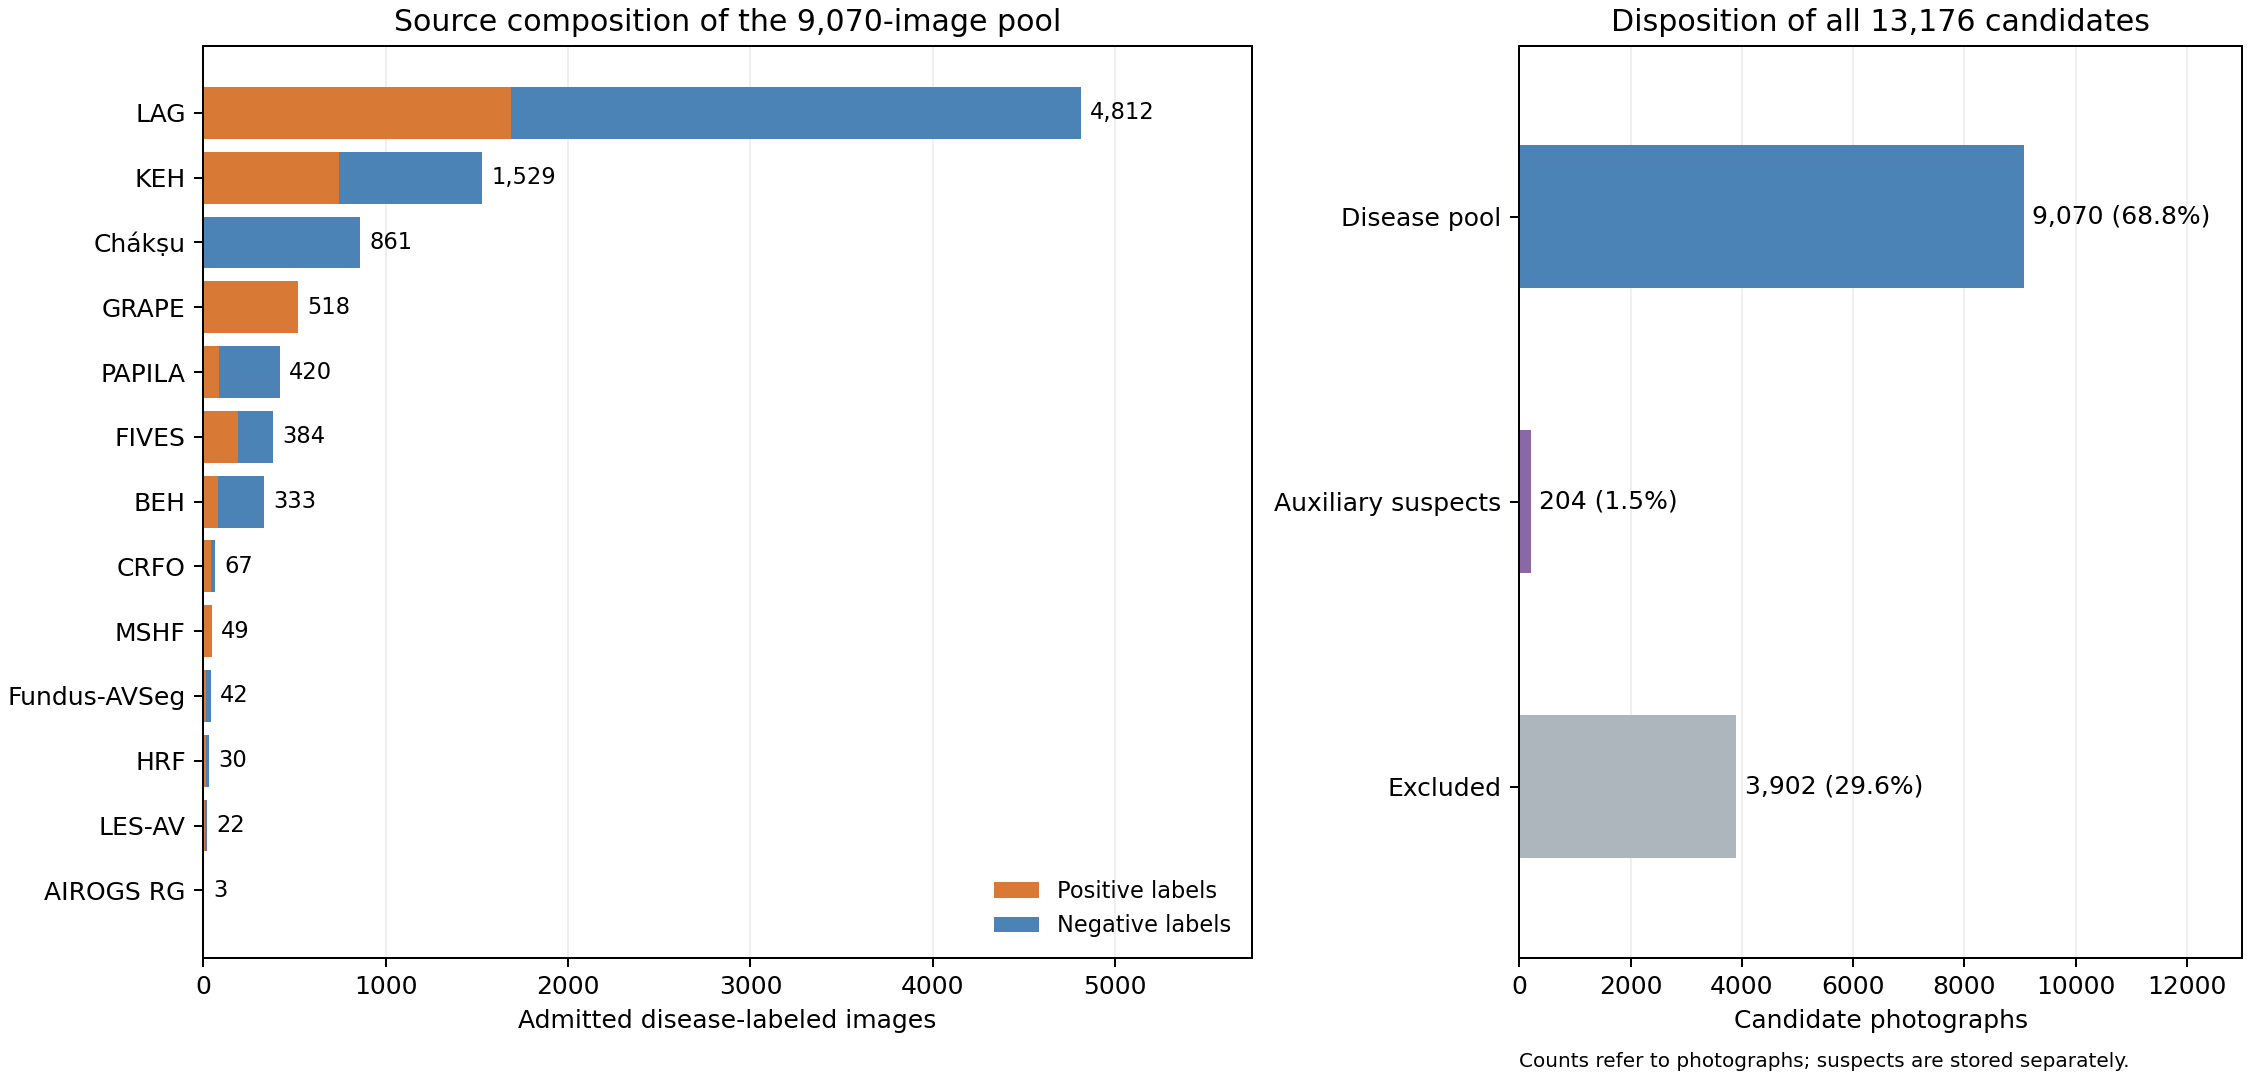
\includegraphics[keepaspectratio,alt={Audit disposition and source composition of admitted photographs}]{admission-and-sources.png}}
\caption{Audit disposition and source composition of admitted
photographs}
\end{figure}

Figure 2 shows positive and negative counts by source in the 9,070-image
disease pool on the left. LAG, KEH, and Chákṣu contribute 7,202 images
together. The right panel accounts for all 13,176 candidates: 9,070
disease-labeled admissions, 204 auxiliary suspects, and 3,902
exclusions. The two admitted pools are stored separately. Counts come
from the audit summary and expansion-pool release.

\textbf{Original rule development was repaired to 1,220 images and 503
positives.} Confirmed training/model-validation relationships involve
ten images in the previous 1,230-image set; these were removed by
identity and saved predictions filtered accordingly. The later four-arm
experiment uses 2,053 joint rule-development images, including these
1,220 originals.

\textbf{Real poor-quality positives total 146.} Among admitted
positives, 99/191 FIVES images have at least one poor official quality
dimension and 47/49 MSHF images have poor overall quality. The two
definitions remain separate, and both original official and
majority-vote MSHF grades are retained. Of the 3,446 positives, 3,443
use source-defined glaucoma diagnoses and three use AIROGS RG referral
labels. Image counts, patient groups, and clinical definitions are
separate manifest fields.

LAG's positive folder retains its name suspicious\_glaucoma; mapping
follows the specialist clinical definition in section 3.1 of the
original CVPR paper. BEH and KEH conflicting-image groups are excluded.
PAPILA and Chákṣu suspects retain their categories. FIVES glaucoma
supervision uses explicit disease labels, while diabetic-retinopathy and
macular-degeneration categories retain their original labels. The two
RIM-ONE partitions organize the same 485 photographs.

KEH provides optic-disc crops, with this imaging domain retained in
disease training. Its quality assessment requires definitions
appropriate to the cropped field. Quality scores for full fundus
photographs and disc crops are interpreted separately.

LAG and GRAPE originate at the same hospital, and confirmed same-eye or
same-photo relationships also connect GRAPE/FIVES, FIVES/Fundus-AVSeg,
and FIVES/MSHF. The five sources are grouped jointly by known patients
and image relationships before allocating training, checkpoint
validation, and rule development. Unknown patient identities use
image-group evaluation; external evaluation holds out complete source
families. GRAPE and the admitted MSHF subset contain only positives and
support detection or miss counts. AUROC and specificity require
corresponding negatives.

\subsection{4. Fundus degradation methods and their
use}\label{fundus-degradation-methods-and-their-use}

At the review stage, the disease pipeline padded to a square, resized to
320×320, and used horizontal flips. The original quality model used
384×384. The November 11 stress pilot used 179 AIROGS, ODIR, and Kaggle
development originals, including 83 positives. At display threshold 0.5,
8/83 positives fell below threshold on originals, 27/83 under stronger
blur, and 20/83 under stronger darkening. Four conditions produced 716
image versions, measured on the same 179 originals. This development
result motivates defocus and exposure experiments.

\Needspace{10\baselineskip}
\begin{longtable}[]{@{}
  >{\raggedright\arraybackslash}p{(\linewidth - 4\tabcolsep) * \real{0.3333}}
  >{\raggedright\arraybackslash}p{(\linewidth - 4\tabcolsep) * \real{0.3333}}
  >{\raggedright\arraybackslash}p{(\linewidth - 4\tabcolsep) * \real{0.3333}}@{}}
\toprule\noalign{}
\begin{minipage}[b]{\linewidth}\raggedright
Work
\end{minipage} & \begin{minipage}[b]{\linewidth}\raggedright
Fundus mechanism and actual release
\end{minipage} & \begin{minipage}[b]{\linewidth}\raggedright
Project use
\end{minipage} \\
\midrule\noalign{}
\endhead
\bottomrule\noalign{}
\endlastfoot
\href{https://arxiv.org/abs/2005.05594}{CoFe-Net, 2020/TMI 2021} &
Uneven illumination, halos, local shadows, artifacts, and defocus;
generation scripts released & First physical reference for a replayable
implementation; old scripts contain Python 3 floating-point random-bound
and spot-replay errors \\
\href{https://arxiv.org/abs/2203.07737}{ArcNet},
\href{https://arxiv.org/abs/2206.04684}{SCR-Net, 2022} & Cataract
opacity and scattering; simulation scripts released & A separate
degradation family, preserving disc assessability; target adaptation
performed on development data \\
\href{https://arxiv.org/abs/2201.00466}{RFormer, 2022} & Restoration
using 120 real low/high-quality repeat pairs & Real repeat-photography
calibration and restoration comparison \\
\href{https://arxiv.org/abs/2309.00885}{GFE-Net, 2023} & High-frequency
structure preservation and unknown degradation; generic scripts released
& Reference for degradation families and structural constraints \\
\href{https://arxiv.org/abs/2409.12377}{FD3, 2024} & Paper describes
clinically calibrated haze/blur/noise/shadow synthesis & Author
repository supplies restoration code and weight links; the full
synthesis program is unavailable \\
\href{https://arxiv.org/abs/2411.12278}{Catintell, 2024} & Learns real
cataract degradation style & Inference and weight links released; full
synthesis training not public in this review \\
\href{https://arxiv.org/abs/2409.07862}{Contextual-OT},
\href{https://arxiv.org/abs/2409.10966}{CUNSB, 2024} & Unpaired
restoration with contextual or vessel-curve constraints; code available
& Restoration ablation, with separate disc and diagnostic validation \\
\href{https://arxiv.org/abs/2411.01403}{TPOT, 2024/2025},
\href{https://arxiv.org/abs/2511.18763}{VAOT, 2025} &
Vessel-topology-constrained restoration & No complete executable release
in checked repositories; not ready components \\
\href{https://arxiv.org/abs/2505.01831}{MTRL-FIE, 2025} & Wavelet,
multi-scale, and lesion features; training and degradation code & Recent
research comparator without an explicit README weight-download entry \\
\href{https://arxiv.org/abs/2502.19153}{RetinaRegen, 2025} & Readability
classification and diffusion restoration, mainly synthetic validation &
Executable author release not verified; real disc/cup preservation
requires separate evaluation \\
\href{https://arxiv.org/abs/2601.13417}{SGW-GAN, 2026} & Restoration
preserving within-disease structure & Adopt task-preservation
evaluation; a complete public implementation was not verified \\
\href{https://arxiv.org/abs/2604.15723}{Handheld diffusion autoencoder,
2026} & Handheld reflection, exposure, and motion-blur restoration &
Relevant to low-resource photography; not run in this project \\
\href{https://arxiv.org/abs/2604.03806}{EyeBench-V2, 2026},
\href{https://arxiv.org/abs/2609.20222}{TSMSA-Net, 2026} & Task/expert
evaluation and two-stage cataract restoration, respectively & Add
glaucoma and optic-disc evaluation; TSMSA uses Kaggle/ODIR and evaluated
within the same sources \\
\end{longtable}

The table distinguishes proposed methods, browseable code, complete
generators, and executed weights. The subsequent
\href{../training-results/degradation-audit.en.md}{degradation audit}
records actual downloads and executions. Restoration can alter cup/disc
edges, color, and fine vessels, so evaluation examines clarity,
diagnostic structures, and disease predictions together. Current
experiments prioritize augmentation with explicit, reproducible
parameters.

\subsection{5. Mixed degradation training and quality
supervision}\label{mixed-degradation-training-and-quality-supervision}

Patient and image grouping precedes allocation. Variants are generated
online inside training groups and inherit their original group.
Application probability is independent of disease label, with actual
applications checked by source and class.

The design compares degradation probabilities of 0\%, 30\%, and 50\%
under common initialization, grouping, and optimizer-update budgets.
Mild or moderate changes include exposure, smooth uneven illumination,
defocus, slight motion, noise, compression, and slight scattering. Use
mainly one family at a time, combining at most two changes. Spatial
severity follows retinal-field diameter, and padding, resizing, and
degradation order are recorded. Blur parameter five at a 512-pixel
reference field and brightness multiplier 0.4 are stronger stress
conditions.

HRF same-eye defocus repeats, Real Fundus pairs, and FIVES/MSHF quality
labels check parameter ranges. Assessability concerns visibility of
cup/disc boundaries and diagnostic evidence. Images with an obscured
disc or insufficient diagnostic evidence support repeat-photography,
rejection, and referral evaluation, while retaining disease metadata.

Quality supervision follows the exact image version. Frozen-teacher
quality targets (teacher\_q) are bound to original-image contents;
degraded versions require newly obtained teacher scores or human grades.
The first degradation experiment augments disease training, while
quality supervision is separately evaluated on actual variants and real
poor-quality images.

Every arm shares fixed originals, real poor-quality cases, and
unassessable groups. Synthetic conditions use paired comparisons on the
same photographs, with patient or linked-group resampling for intervals.
Primary outcomes include real poor-quality positive sensitivity,
sensitivity at fixed specificity, AUPRC, probability calibration, and
residual misses at matched review volume. AUPRC is the area under the
precision--recall curve and depends on positive prevalence; interpret it
within the same source. Real-photo and synthetic-stress outcomes are
reported separately.

\subsection{6. Training size and evaluation
precision}\label{training-size-and-evaluation-precision}

The binary EfficientNet-B0 used here has 4,008,829 parameters and
ImageNet initialization. Required training data depends on source
coverage, cases, and development performance. Nested grouped learning
curves compare 25\%, 50\%, 75\%, and 100\% of training groups, each with
three seeds. Preserve source and disease strata and complete
patient/image groups, training from common initialization.

All sizes share maximum update budgets and validation cadence. Record
actual updates, selected checkpoints, repeated draws, and distinct-image
coverage. Choose training size using development ranking, sensitivity,
and real poor-quality performance. Allocate evaluation roles before
training a new release; images learned by existing weights remain
development or new-model training data.

\Needspace{10\baselineskip}
\begin{longtable}[]{@{}
  >{\raggedright\arraybackslash}p{(\linewidth - 4\tabcolsep) * \real{0.3000}}
  >{\raggedleft\arraybackslash}p{(\linewidth - 4\tabcolsep) * \real{0.4000}}
  >{\raggedright\arraybackslash}p{(\linewidth - 4\tabcolsep) * \real{0.3000}}@{}}
\toprule\noalign{}
\begin{minipage}[b]{\linewidth}\raggedright
Independent-positive precision planning
\end{minipage} & \begin{minipage}[b]{\linewidth}\raggedleft
Approximate positives
\end{minipage} & \begin{minipage}[b]{\linewidth}\raggedright
Interpretation
\end{minipage} \\
\midrule\noalign{}
\endhead
\bottomrule\noalign{}
\endlastfoot
Sensitivity near 95\%, margin ±5 percentage points & 73 &
Independent-binomial precision approximation \\
Sensitivity near 95\%, margin ±3 percentage points & 203 & Same
approximation \\
Sensitivity near 95\%, margin ±2 percentage points & 457 & Same
approximation \\
Zero misses, one-sided 95\% miss-rate upper bound near 5\% & 59 &
Zero-event binomial bound \\
Zero misses, one-sided 95\% miss-rate upper bound near 2\% & 149 & Same
bound \\
Zero misses, one-sided 95\% miss-rate upper bound near 1\% & 299 & Same
bound \\
\end{longtable}

These counts plan estimation precision; actual grouped data use
linked-group resampling. Comparing review strategies also requires a
paired power calculation based on discordant decisions in development
cases.

Prioritize about 200 independent positives in a main cohort with
compatible clinical definitions and add real poor-quality strata. New
sources with patient identifiers can start allocation planning at 60\%
training, 10\% checkpoint validation, 10\% rule development, and 20\%
testing, followed by checks of positive counts per role. The five
associated sources are grouped jointly. ACRIMA and HYGD retain
external-test roles. Models, degradation parameters, classification
thresholds, and review rules are determined during development.

\subsection{7. Experiment progression and
evidence}\label{experiment-progression-and-evidence}

This review delivered the expansion pool, label/group audits,
degradation research catalog, and
\href{experiment-proposal.json}{experimental design}. Later on the same
day, joint allocation, four 1,200-update training arms, and development
predictions completed. Grouped learning curves, additional seeds, locked
review rules, and final testing remain subsequent work. See the
\href{../training-results/training-results.en.md}{training report} and
\href{../experimental-analysis/experimental-analysis.en.md}{paired
analysis} for results.

\href{../../../../data/audit/data_expansion_20261113/public_dataset_review.md}{Public-data
review} ·
\href{../../../../data/audit/data_expansion_20261113/local_decisions.csv}{Per-image
audit} ·
\href{../../../../data/audit/data_expansion_20261113/local_summary.json}{Audit
summary and input hashes} ·
\href{../../../../data/prepared/expansion_20261113/README.en.md}{Expansion
pool} ·
\href{../../../../data/audit/data_expansion_20261113/degradation_review.md}{Degradation
literature and code} ·
\href{../../../../data/audit/data_expansion_20261113/degradation_sources.json}{Release
evidence} · \href{development_analysis.json}{Development statistics} ·
\href{analyze_splits.py}{Statistics and Figure 1} ·
\href{plot_admission.py}{Figure 2 script}.

Both languages and figures use common audit and statistical inputs. The
LaTeX sources for the PDFs are retained beside the reports.

\end{document}
